\section{High Level Trigger}
responsible editor: Jyothsna\\
%add documentation about btag mu triggers and possibly some comments on the btag IP triggers used in PAGS.
Technical implementation to use b-tagging at High Level Trigger (HLT) enviromnent
exists since few years \textbf{FIX ME add 2006 and 2007 references here}.
These implementations exploit couple of properties of jets originating 
from b-quarks namely semi-leptonic decays and long lifetime. ``BTagMu'' 
implementation makes use of semi-leptonic b-decays and tags jets at
HLT containing muons associated to them. Lifetime based b-tagging
implementation referred to as ``BTagIP'' implementation relies mostly on 
offline equivalent of Track Counting High Efficiency algorithm for
tagging the jets at HLT. 

Implementation details of ``BTagMu'' and ``BTagIP'' along with the 
triggers developed for calibration and physics use cases is 
presented in the next sections.

\subsection{BTagMu HLT implementation and use cases}
Events containing a $\mu$ associated with a jet can be used to the
measure the b-tag performance from data. Since only paths using BTagMu
implementation are the b-tag calibration paths, these are
explicitly mentioned in the below description of the implementation.
The Level~1 seeds for these paths require a muon and a jet at Level~1
with $E_T$ cuts specific to each designed HLT path and are listed in 
Table \ref{btagmu}.

\begin{itemize}
\item Level-2: In 2011 Anti $k_T$ corrected calo jets are used as
  Level-2 jets. In order to reduce the HLT rates dijets are required
  at Level-2 with varying jet $E_T$ thresholds. These jet $E_T$ cuts
  are tuned to have enough statistics available offline to derive the
  efficiency and scale factors in various offline jet $E_T$ and $\eta$
  bins. In the recent data taking 20~GeV, 40~GeV, 70~GeV and 110~GeV
  are chosen as the thresholds.
\item Level-2.5: The soft lepton b-tagging algorithm is run on the 4 highest $E_T$ jets in the event
  with $E_T$ threshold chosen same as the $E_T$ cut on jets at
  Level-2. Level-2 muons, reconstructed using muon detector hits,
  are required to be near one of these 4 highest $E_T$ jets, $\Delta R(\mu, jet)
  ~<~0.4$, using the Soft Lepton b-tagging algorithm. Events pass if
  at least one jet is soft mu-tagged.
\item Level-3: Refined tracking is used to reconstruct Level-3
  muons. Only those Level-3 muons which pass $\mu~p_T~>5~GeV$ and have
  $>~0$ number of hits are used to select muon-in-jets with $\Delta R(\mu, jet)
  ~<~0.4$ requirement using the Soft Lepton b-tagging algorithm. Events pass if
  at least one jet is soft mu-tagged.
\end{itemize}

The Soft Lepton b-tagging algorithm used in both Level-2.5 and Level-3 make
use of the same methods used in the offline reconstruction and they
differ in muon and jet inputs at HLT wrt Offline.

The names of the ``BTagMu'' based triggers along with the Level-1
seeds are listed in Table \ref{btagmu}.

\begin{table}[htbp]
\begin{center}
\begin{tabular}{|c|c|c|c|}
\hline
\texfbf{Path name} & \textbf{Level-1 seed} & \textbf{HLT prescale} & \textbf{Rate @1E33}\\
\hline
HLT\_BTagMu\_DiJet20\_Mu5 & L1\_Mu3\_Jet16 & 350 & 1.62~Hz \\
HLT\_BTagMu\_DiJet40\_Mu5 & L1\_Mu3\_Jet20 & 100 & 1.32~Hz \\
HLT\_BTagMu\_DiJet70\_Mu5 & L1\_Mu3\_Jet28 & 15 & 1.36~Hz \\
HLT\_BTagMu\_DiJet110\_Mu5 & L1\_Mu3\_Jet28 & 2 & 1.62~Hz \\
\hline
\end{tabular}
\end{center}
\caption{}
\label{btagmu}
\end{table}

The offline selection required two jets of $\pt > 30\GeV$ and $|\eta|
< 2.4$ in order to stay within the tracker acceptance and in the
\pt\ range where b-tagging is typically applied. In order to increase 
the purity in ${\mathrm B} \to \mu + {\mathrm X}$ decays the event had 
to contain exactly one muon of $\pt > 6\GeV$ and $|\eta| < 2.4$ with
the following additional quality criteria:
\begin{itemize}
\item the muon was reconstructed as a ``GlobalMuon'' with at least one valid muon hit, more than one matching segment in the muon chambers and a $\chi^2/{\mathrm ndof}<10$;
\item the corresponding inner track had $>10$ hits with at least one hit in the pixel system and a $\chi^2/{\mathrm ndof}<10$;
\item the $z$-distance between the reference point of the muon and the selected primary vertex was $< 1$cm.
\end{itemize}
The muon had to be in a cone defined by $\DR < 0.4$ around the associated jet (``\muonjet'').

Turn on curves for the different BTagMu triggers have been computed by scaling the pT spectra for
the data collected by each trigger by its integrated luminosity, and dividing the so obtained
distribution by the one of the HLT\_BTagMu\_DiJet20\_Mu5 trigger. The turn on curve for
this last trigger has been computed by taking the pT spectrum of the muon-jetsin data collected
by the HLT\_Mu5 trigger as a reference. All these turn on curves are
shown in Fig. ~\ref{btagmuturnon}.

\begin{figure}[h!]
\centering
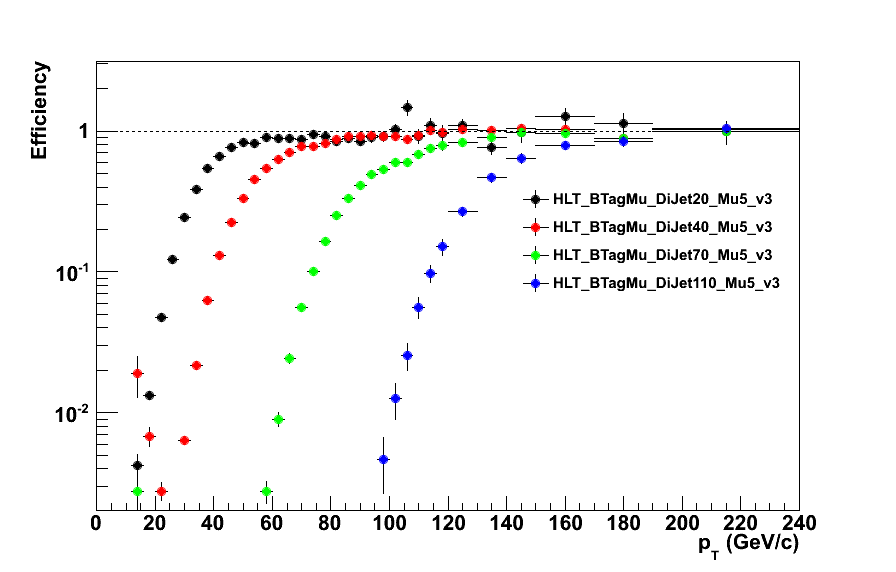
\includegraphics[width=0.65\textwidth]{figures/BTagMuTriggerTurnOn.png}
\caption{Turn on curve of all the above four paths using 2011 data}
\label{fig:btagmuturnon}
\end{figure}


\subsection{BTagIP HLT implementation and use cases}
Many standard model and exotic physics channels contain b jets in the
final state. By explicitly requiring b-tagged jets in the HLT paths 
for these physics channels, one can lower the jet $E_T$ thresholds 
than cutting harder on the jets for rate reduction, increasing the
purity as well as trigger efficiency for these channels.

A generic BTagIP implementation at HLT is described below. This
implementation is adapted to suit the needs of physics channels by the 
trigger developers. The Level-1 seeds are also up to the trigger
developers to choose depending on the physics channel and final state
they are interested in.

\begin{itemize}
\item Level-2: The jet $E_T$ thresholds and the number of jets vary
  depending on the needs of the physics channel.
\item Level-2.5: Tracks are reconstructed using the Pixel Tracker
  alone (each with at least 3 hits), and are then used to reconstruct
  the 1D primary vertex. The b-tag is run on 4-6 highest $E_T$ jets in
  the event with $E_T$ threshold chosen by the trigger developer,
  using the pixel tracks and the primary vertex as input. Most of the
  physics paths use Online Beam Spot in the transverse plane and fast
  estimation in Z as the primary vertex. 3D Primary vertex (PV) can also be
  used as reference. More details about the PV methods usage at HLT
  and the performnace are provide in the next subsection. Jets are
  tagged as b-jets if they have at least 1 or 2 tracks with 3D impact
  parameter significance greater than a threshold value tuned by the
  physics trigger developers. Events pass if at least one or two
  jets are b-tagged.
\item Level-3: Tracks are reconstructed regionally in a cone size
  $\Delta R~=~$ 0.25 either around the jets tagged as b-jets at
  Level-2.5 or around all the Level-2.5 jets. The choice of which jets
  are fed for the regional track reconstruction is also upto the
  developers. The track reconstruction is partial. stopping after 
  8 hits have been assigned to a track. The b-tag uses these tracks
  and the primary vertex reconstructed at Level-2.5. It selects jets
  having at least 2 tracks with 3D impact parameter significance
  greater than a threshold value tuned by the trigger
  developer. Events pass if at least one or two jets are b-tagged.
\end{itemize}

Trigger performance of couple of physics channels using BTagIP are
presented in Fig~\ref{QuadJetturnon} for QuadJet50\_BTagIP trigger path
and Fig~\ref{RA2bturnon} for HT300\_CentralJet30\_BTagIP\_PFMHT55
trigger path as a function of offline b-tag algorithms. 

QuadJet50\_BTagIP trigger path is developed for all hadronic ttbar
final state and to collect the events containing at least four jets at the HLT level with $E_T > 50$ GeV and
amongst at least one of them is required to be b-tagged by TCHE
algorithm at HLT. The cut TCHE cut chosen at HLT level is 2 for this
path and as can be seen in bottom plot in Fig~\ref{QuadJetturnon} the
efficiency is 50\% at offline TCHP value of 2.

SUSY analysis looking at missing $E_T$, jets and b-jet final state and
developed trigger path HT300\_CentralJet30\_BTagIP\_PFMHT55 to collect
such events. Jet with $E_T >$ 30 GeV is required to be b-tagged by
TCHE algorithm at HLT and the cut applied is at 4.

\begin{figure}[h!]
\centering
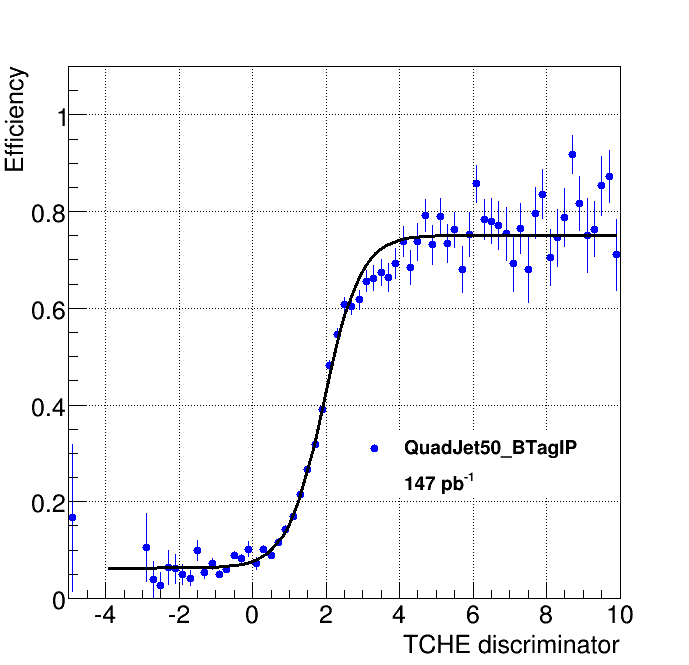
\includegraphics[width=0.5\textwidth]{figures/QuadBTagTCHE_turnOn.png}
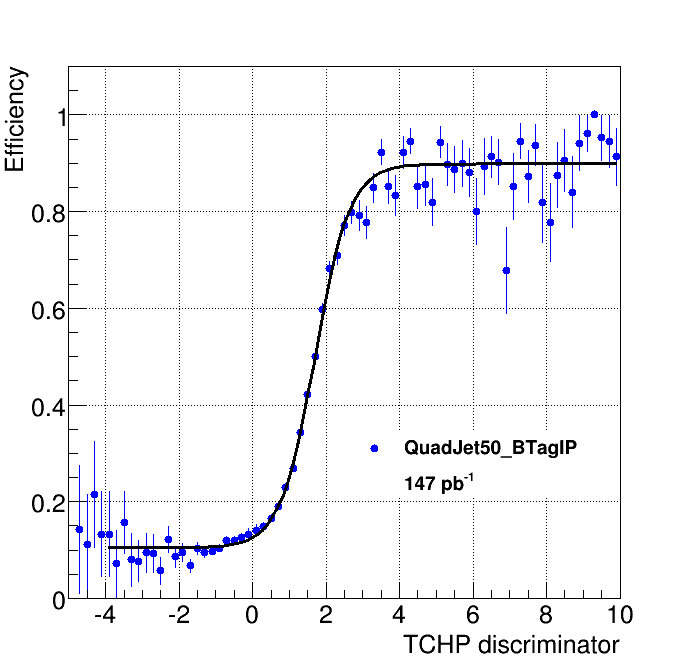
\includegraphics[width=0.5\textwidth]{figures/QuadBTagTCHP_turnOn.png}
\caption{Turn on curve for QuadJet50\_BTagIP trigger as a function of offline TCHE and TCHP
  discriminator obtained using 2011 data}
\label{fig:QuadJetturnon}
\end{figure}

\begin{figure}[h!]
\centering
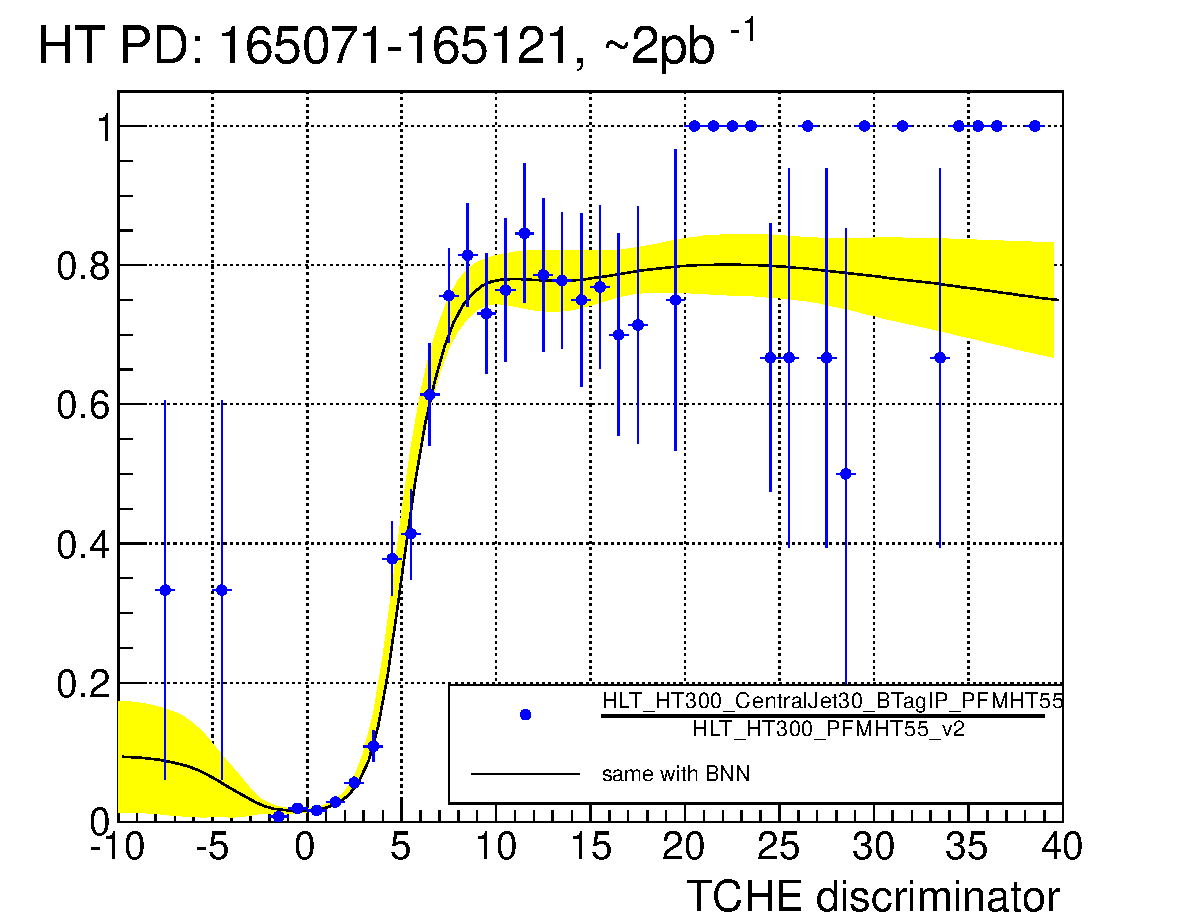
\includegraphics[width=0.5\textwidth]{figures/RA2bSUSY_TCHE_turnOn.pdf}
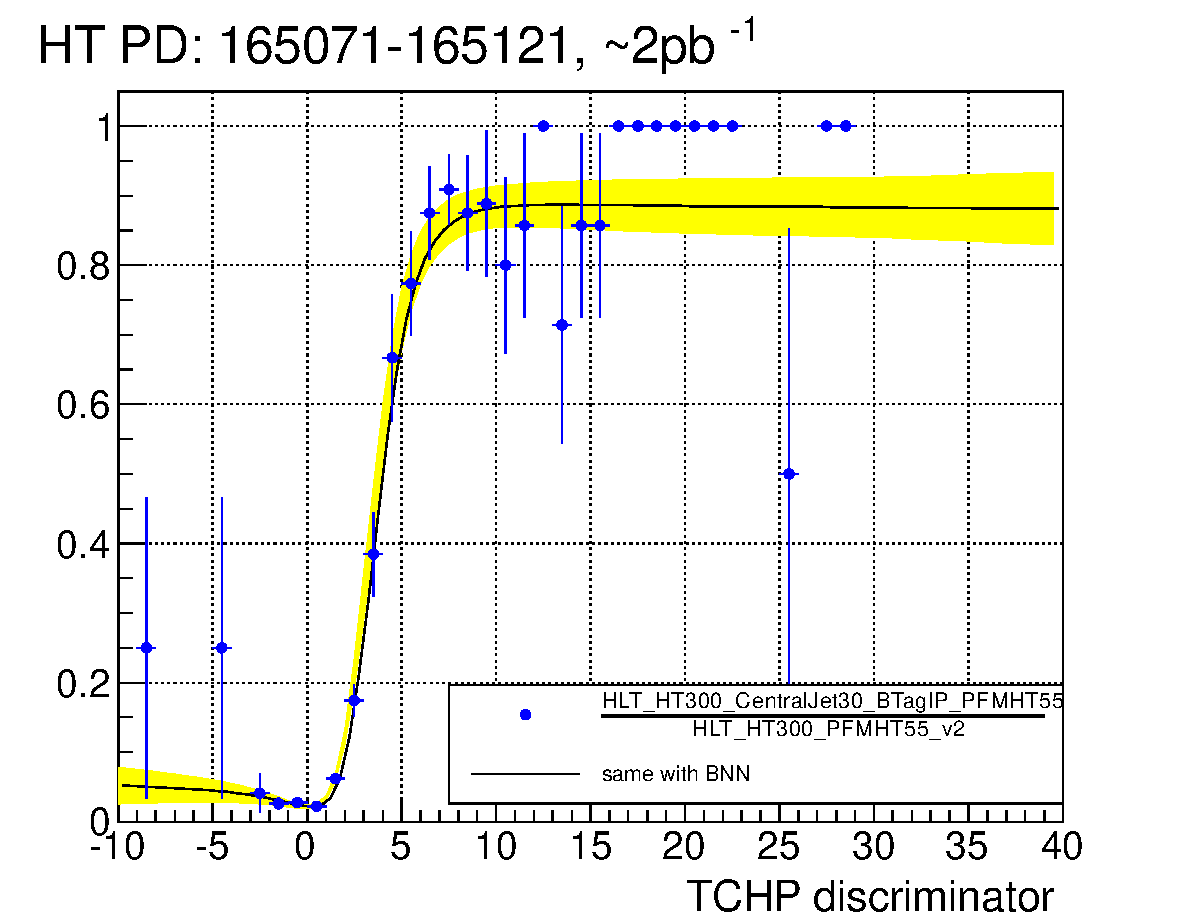
\includegraphics[width=0.5\textwidth]{figures/RA2bSUSY_TCHP_turnOn.pdf}
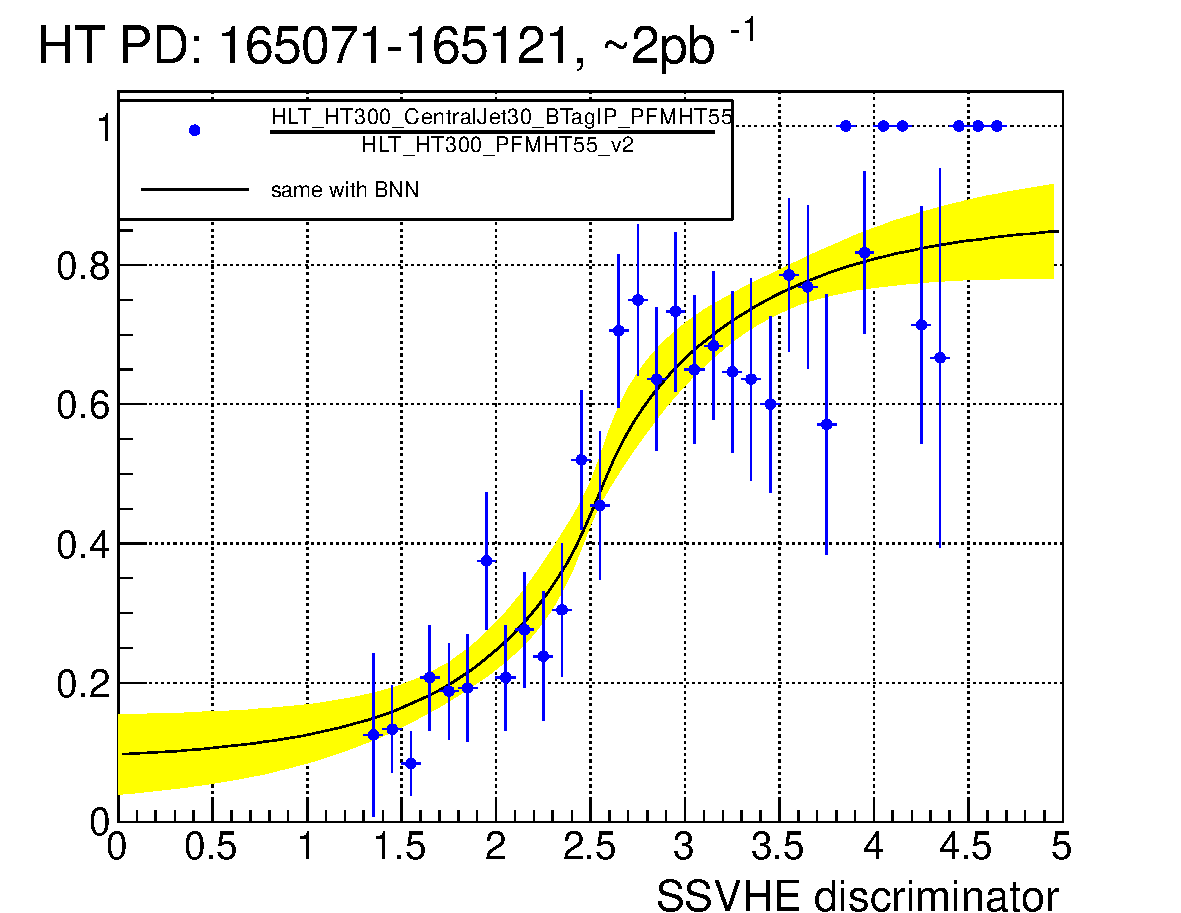
\includegraphics[width=0.5\textwidth]{figures/RA2bSUSY_SSVHE_turnOn.pdf}
\caption{Turn on curve for HT300\_CentralJet30\_BTagIP\_PFMHT55 as a
  function of offline TCHE, TCHP and SSVHE discriminator obtained using 2011 data}
\label{fig:RA2bturnon}
\end{figure}

\subsection{3D Primary Vertex}
responsible editor: Carlotta\\
To limit the CPU timing, the standard High Level Trigger reconstruction performs only a fast partial (1D) estimation of the primary vertex. Prompt pixel tracks are clustered in $z$ and the longitudinal vertex position is determined by the Divisive Vertex Fitter algorithm. The online beamspot is used as rough estimation of the transverse vertex coordinate.\\
%The pixel tracks in the event are clusterized into primary vertex candidates, and the vertex longitudinal position is determined by the Divisive Vertex Fitter as average of the $z$ of tracks in the cluster. A rough estimation of the transverse position is given by the beam spot. 
The full (3D) primary vertex reconstruction, implementing the Adaptive Vertex Fitter, could provide a reliable reference point for the track impact parameter calculation, input to the b-tagging algorithms, in case of movements of the beamspot. This will be crucial, at  high luminosity, for those trigger paths that rely on b-tagging to reduce the rate by a factor greater than 10. To avoid any bias from an incorrect beamspot position, no beam constraint is applied in the vertex fitting procedure.
%No beam constraint is applied, to exclude any bias in case the beamspot position is incorrect.
The Gap clusterizer is used.
To be included in the clusterization, pixel tracks are required to have at least 3 pixel hits, $\chi^{2}/ndof \leq$ 100.0, and transverse impact parameter significance $\leq$ 100.0.
An additional cut on the track momentum can be applied and tuned in order to achieve reasonably good performance with a limited CPU consumption. Tracks that pass the selection are grouped into primary vertex candidates if their $z$ distance to the nearest neighbor is smaller than 1 mm. A reconstructed primary vertex is finally rejected if the transverse distance to the beam is larger than 2 cm. 

The performance of the 3D primary vertex reconstruction, compared to the standard 1D, is evaluated using a Monte Carlo sample of QCD events with parton $p_{T}$ greater than 15 GeV$/c$, with on average 10 pile up events. 
Fig.\ref{efffake} and \ref{res} summarize the results for vertex finding efficiency, rate of fake vertices in the event, transverse and longitudinal position resolution, as a function of the $p_{T}$ cut applied to the pixel tracks.
% track and vertex sim-to-reco association?
%Fig.\ref{eff} shows the primary vertex finding efficiency provided by the 3D algorithm, as a function of the $p_{T}$ threshold applied to the pixel tracks. For the signal vertex, the efficiency is higher than 90\% up to a $p_{T}$ cut of 1.3 GeV$/c$, and is competitive with the performance of the 1D reconstruction, which applies a $p_{T} \geq$ 0.9 GeV selection. The rate of fake reconstructed vertices in the event, as a function of the $p_{T}$ threshold, is shown in Fig.\ref{faker}. For the standard 1D it is measured to be 12.5\%.
\begin{figure}
   \centering
   %%----start of first subfigure----
   \subfloat[]{
        \label{eff}           %% label for first subfigure
        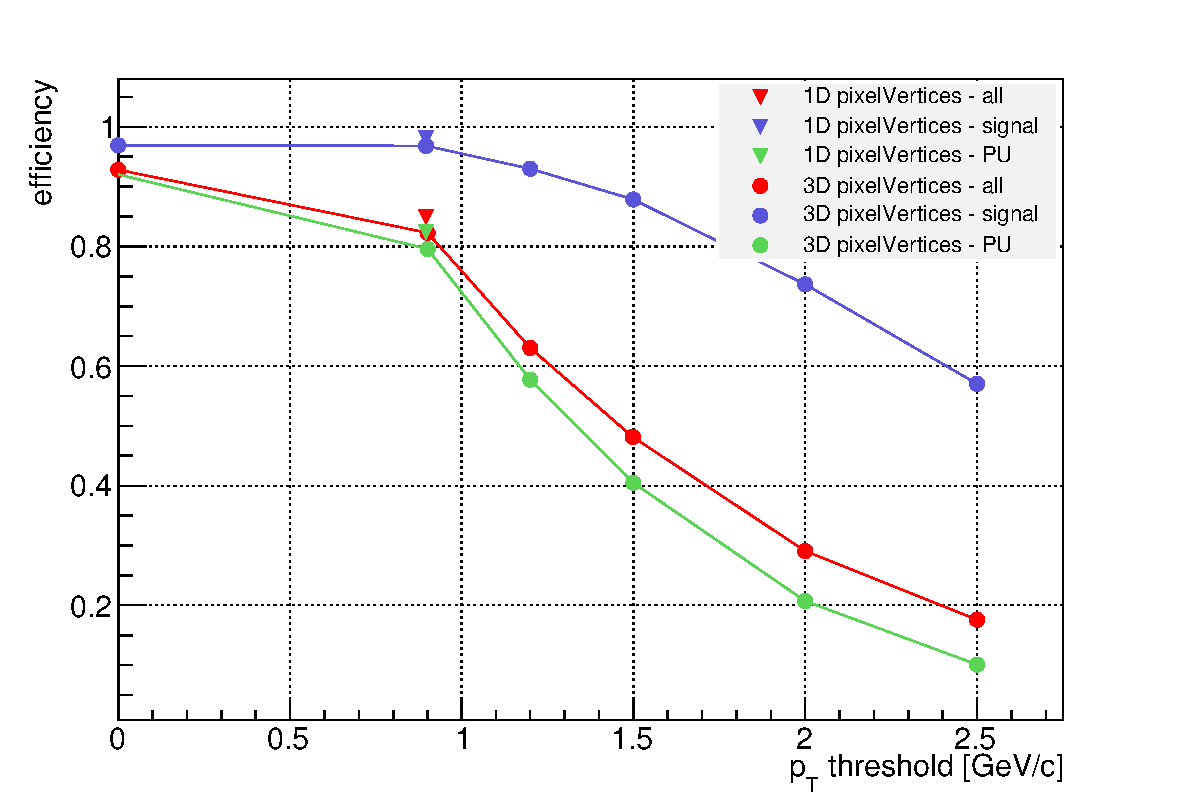
\includegraphics[height=4.7cm]{figures/3DPVeff.pdf}}
   \hspace{0.1cm}
   %%----start of second subfigure----
   \subfloat[]{
     \label{faker}           %% label for second subfigure
        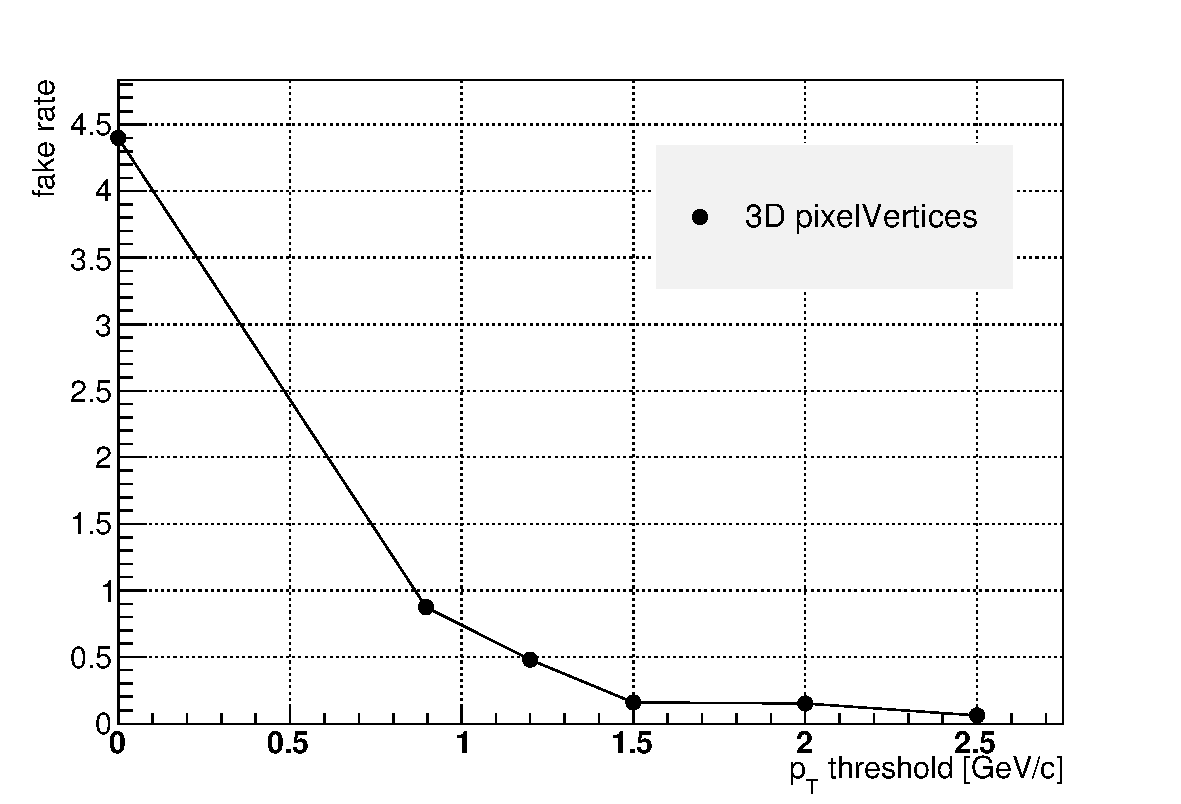
\includegraphics[height=4.7cm]{figures/3DPVfake.pdf}}
   \caption{\small{(a) primary vertex finding efficiency provided by the 3D reconstruction, for all vertices in the event, and separately for signal and pile up vertices, as a function of the $p_{T}$ threshold applied in the pixel track selection. The result for the 1D pixel vertex reconstruction is also shown for a comparison. (b) rate of fake vertices in the event, as a function of the $p_{T}$ threshold. The corresponding fake rate for the 1D reconstruction is 12.5\% for a $p_{T}$ cut of 0.9 GeV$/c$.}}
   \label{efffake}                  %% label for entire figure
\end{figure}
%_________________________________________________________________________________
\begin{figure}
   \centering
   %%----start of first subfigure----
   \subfloat[]{
        \label{resT}           %% label for first subfigure
        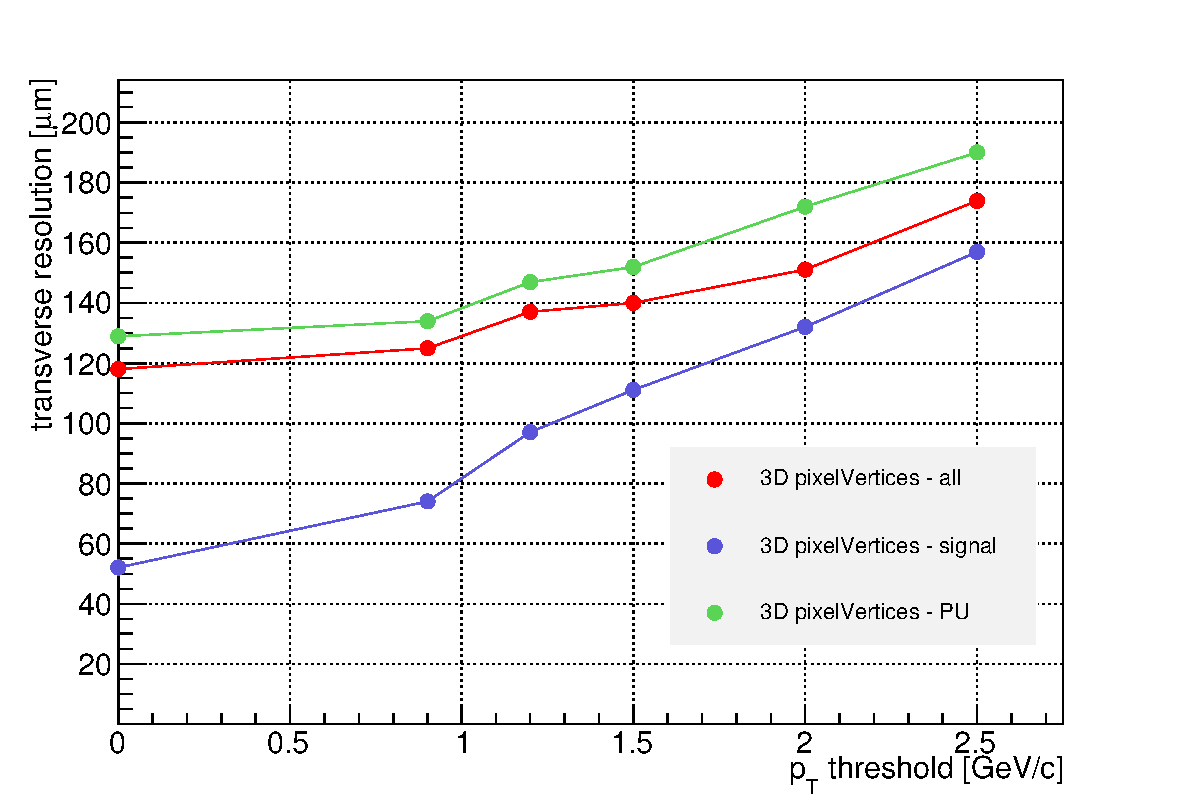
\includegraphics[height=4.7cm]{figures/3DPVresX.pdf}}
   \hspace{0.1cm}
   %%----start of second subfigure----
   \subfloat[]{
     \label{resL}           %% label for second subfigure
        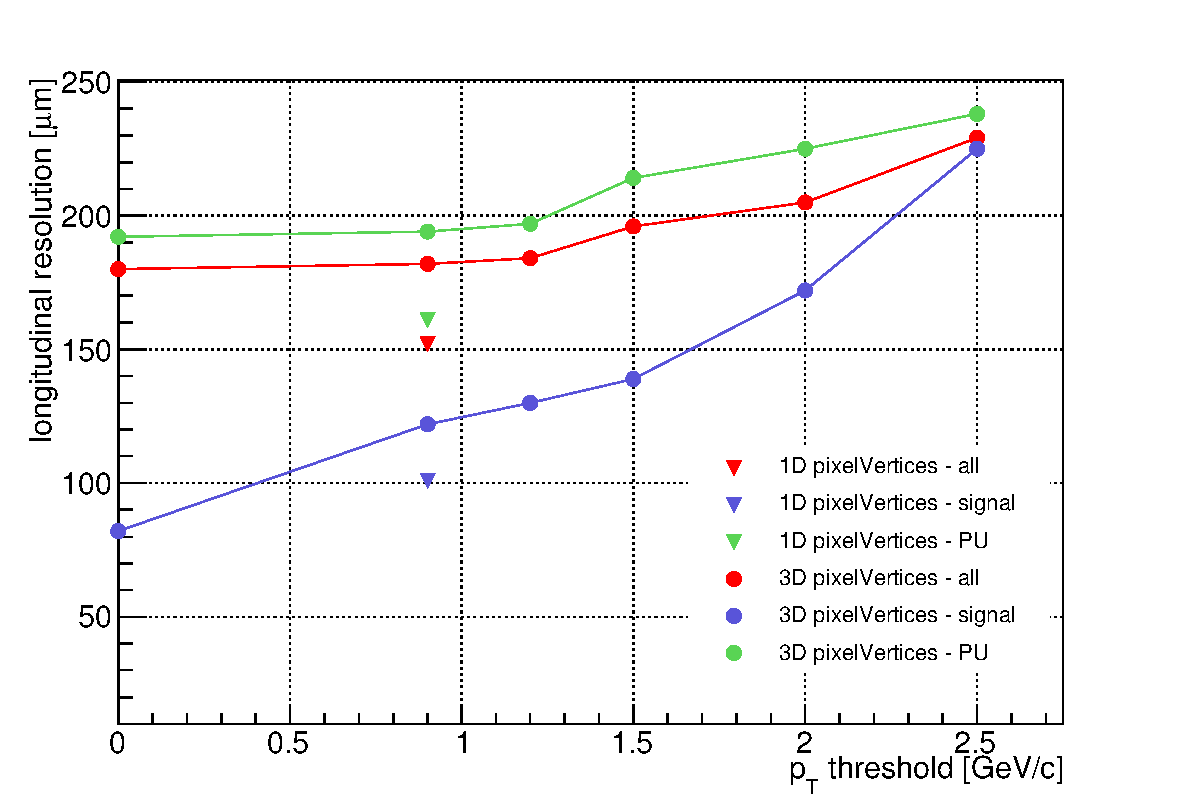
\includegraphics[height=4.7cm]{figures/3DPVresL.pdf}}
   \caption{\small{(a) transverse and (b) longitudinal 3D primary vertex position resolution as a function of the $p_{T}$ threshold applied in the pixel track selection. In (b) the result for the 1D reconstruction is also shown for comparison.}}
   \label{res}                  %% label for entire figure
\end{figure}
From Fig.\ref{eff} it is evident that a working point for this algorithm should be chosen in the region up to about 1.2 GeV$/c$, where the signal vertex efficiency is higher than 90\%, and competitive with the 1D reconstruction. The fake rate in this range is between 4.5\% and 0.5\%, to be compared to 12.5\% that we obtain for the 1D reconstruction. For the signal vertex, the longitudinal position resolution ranges between 80 and 120 $\mu$m. The transverse resolution is between two and four times worse than the beamspot width (about 25 $\mu$m), which is the limitation of the 1D algorithm. This should still assure sufficiently good b-tagging performance for the purpose of the online event selection. \\
A summary of the 3D vertex reconstruction performance is given in Table \ref{summary}, together with an estimation of the running time (CPU) of the module. 
\begin{table}[htbp]
\begin{center}
\begin{tabular}{|c|c|}
\hline
$p_{T}$ threshold (GeV$/c$) & running time (ms) \\
\hline
no threshold & 32.6 \\
0.9 & 15.5 \\
1.2 & 10.0 \\
1.5 & 7.1 \\
2.0 & 4.8 \\
2.5 & 3.9 \\
\hline
\end{tabular}
\end{center}
\caption{Running time (CPU) of the 3D primary vertex producer module as a function of the $p_{T}$ threshold applied in the pixel track selection.} 
\label{summary}
\end{table}
